\begin{example} \label{eg:6.4.1} % EXAMPLE
A thin bar occupies the interval $0 \leq x \leq 2$ and it has a density in kg/m of $\rho(x) = 1+ x^2$. Find the mass of the bar. 

\solution
The mass of the bar in kilograms is 
\begin{align*}
	m &=	\int_a^b \rho(x) \ dx \\
		&=	\int_0^2 (1+x^2) \ dx \\
		&= 	\left(x+\frac{x^3}{3} \right) \Big|_0^2 \\
		&= \frac{14}{3} \text{kg}.
\end{align*}

\end{example}

%\begin{marginfigure}[-8cm] %MARGIN FIGURE
%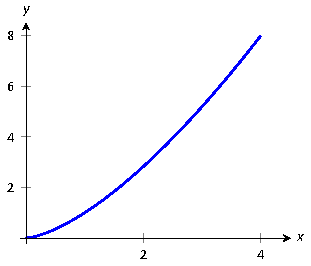
\includegraphics{figures/figarc1}
%\caption{A graph of $f(x) = x^{3/2}$ from Example~\ref{eg:6.3.1}.} \label{F:6.3.Ex1}
%\end{marginfigure}

